% ============================================================================
\section{Introduction}
\label{ch:introduction}
% ============================================================================

\subsection{Context}

The Robot Operating System 2 (ROS2)~\cite{macenski2022ros2} has become as the de facto standard platform for robot development, providing a comprehensive and flexible messaging communication mechanism that enables efficient information transmission both within and between robots. As robotic systems are increasingly deployed across diverse domains including manufacturing, healthcare, aerospace exploration, and autonomous vehicles, ensuring their reliable and correct operation becomes vital.

Robots operating in complex and dynamic environments frequently encounter unexpected events and emergent situations that cannot be fully enumerated during the design phase. When environmental changes and operational states cannot be perceived timely, serious consequences often result. Furthermore, many robots today are controlled and make decisions by AI, the complexity of AI models is a black box for testing. These all make it difficult to use formal methods alone to prove that robots will always operate correctly, thus runtime monitoring as a necessary complement to design-time verification.

Runtime monitoring addresses this gap by continuously collecting robot runtime states, and enabling real-time observation of system behavior. Unlike exhaustive enumeration of all possible system states, runtime monitoring only analyzes data generated during system execution, thus avoiding the state space explosion problem inherent in model checking approaches.

\subsection{Problem Statement}

A comprehensive monitoring framework for ROS2 can be defined as a layered architecture:

\begin{itemize}[leftmargin=*]
    \item \textbf{Bottom Layer:} The capability to observe and collect observations from ROS2 systems
    \item \textbf{Middle Layer:} The ability to abstract and represent collected data at different levels
    \item \textbf{Top Layer:} The ability to evaluate observations using various domain specific languages
\end{itemize}

This project focuses on the foundation layer, i.e. the capability to systematically collect observations from ROS2 systems and generate the corresponding monitoring infrastructure based on user-defined configuration. This bottom-up approach establishes essential groundwork, upon which higher-level abstraction and evaluation layers can be built in future work.

\subsection{Research Questions}
Given that there is currently no unified monitoring foundation that addresses all communication primitives. In particular, monitoring approaches for Actions remain underexplored. This research aims to bridge these gaps by designing a Foundation Layer that enables developers to declaratively specify and automatically generate monitoring infrastructure that is both comprehensive and architecturally flexible. To guide this work and validate its effectiveness, the following research questions are posed:

\subsubsection{RQ1}
What monitoring capabilities currently exist in ROS2 systems across different levels, and what are the gaps regarding observable elements?

\subsubsection{RQ2}
How can all observable elements and configuration options in ROS2 be organized into a unified model to represent monitoring options and requirements?

\subsubsection{RQ3}
How can we automatically generate the monitoring infrastructure based on the unified model?

\subsubsection{RQ4}
What are the performance impacts and trade-offs of different monitoring architectures?

\subsection{Approach}

\subsubsection{Approach for RQ1}
I will perform a literature and tool review. I will compare existing ROS2 monitoring methodologies, including Node-Level, Network-Level, and System-Level approaches, and identify the gaps.

\subsubsection{Approach for RQ2}
I will develop a Feature Tree, a model which represents universal monitoring options and limitations across different configurations in ROS2 systems.

\subsubsection{Approach for RQ3}
I will develop a Code Generator that takes the Feature Tree configuration set by users, detects context of ROS2 systems at runtime, and automatically generates the ROS2 monitors according to configuration.

\subsubsection{Approach for RQ4}
I will deploy the generated monitors on a specific ROS2 system in a Gazebo simulation and measure the CPU, memory, and latency overhead under different architecture setups.

\newpage

% ============================================================================
\section{ROS2 Background}
\label{ch:ros2background}
% ============================================================================

\subsection{Nodes}
Nodes~\cite{ros2nodes} are the most fundamental modules in the ROS system. Each node designed to perform a single, modular task, such as adjusting the angle of a steering drive shaft or processing temperature sensor data. A ROS system typically consists of many nodes working collaboratively. Each node has a unique identifier to ensure correct routing and prevent conflicts during data exchange between nodes. The methods of information exchange between nodes are described below.

\subsection{Topics}
Topics~\cite{ros2topics} serve as the hub for information exchange between nodes, and represent one of the primary ways for nodes to exchange information. They adopt a publish-subscribe pattern where nodes can act as publishers to send data to a topic or as subscribers to receive data from a topic. There is no limit to the number of topics a node can subscribe to, meaning topics are not restricted to point-to-point communication but can support one-to-many, many-to-one, or many-to-many relationships. Messages transmitted through topics are typically stable information streams with fixed frequencies. For example, a control node may send a message containing linear velocity v to a topic named /cmd vel every 100ms for 1 second. The node responsible for actually controlling the robot subscribes to this topic, enabling the robot to move forward in its current direction at velocity v for 10 iterations.

\subsection{Services}
Services~\cite{ros2services} are another form of communication between nodes. Unlike topics, services adopt a call and-response model rather than a publish-subscribe model. A client node sends a request to a service,which forwards it to a server node, and then transmits the server node's response back to the client node in the reverse direction. It is a unidirectional, one-time communication method. Similar to typical client-server models, multiple client nodes can use the same service, but only one server node can provide services to handle requests and generate responses for that service.

\subsection{Actions}
Actions~\cite{ros2actions} are a communication method that combines the publish-subscribe model with the request response model, suitable for executing tasks that require an extended period to run. During execution, actions can continuously generate feedback messages reporting status and can be interrupted. Action Client and Action Server nodes communicate Goal and Result information through request-response interactions at the start and end of an action, while the Server node continuously publishes feedback during execution, enabling the Client node to monitor the execution status. Figure~\ref{fig:action} illustrates the Action execution process.

\begin{figure}[H]
    \centering
    
\includegraphics[width=0.85\linewidth]{Image/Actions.png}
    \caption{Action}
    \label{fig:action}
\end{figure}

\subsection{Middleware}
Middleware~\cite{ros2middleware} is positioned below the user layer and ROS framework but above the operating system, hiding detailed hardware device information from the application layer. DDS for real-time systems is an Object Management Group machine-to-machine standard that aims to enable dependable, high-performance, interoperable, real-time, scalable data exchanges using a publish–subscribe pattern. Since ROS systems extensively employ publish-subscribe mechanisms for communication,DDS is highly suitable as middleware for ROS data communication. ROS uses DDS as its default middleware, supporting eProsima Fast DDS, RTI Connext DDS, Eclipse Cyclone DDS,and GurumNetworks Gurum DDS. Their performance varies across different environments.

\newpage

% ============================================================================
\section{Literature Review and Feature Model}
\label{ch:litreview}
% ============================================================================

\subsection{What Can Be Observed}
Identify and document observable elements in ROS2, including:

\begin{itemize}[leftmargin=*]
    \item \textbf{Topics:} Publish-subscribe communication channels for streaming data between nodes.
    \item \textbf{Services:} Request-response communication for synchronous operations.
    \item \textbf{Actions:} Long-running tasks with goal, feedback, and result communication.
    \item \textbf{Parameters:} Runtime-configurable node settings.
    \item \textbf{Node States:} Changes of Life cycle of Nodes, from Unconfigured to Finalized.
    \item \textbf{QoS Events:} Events related to Quality of Service.
\end{itemize}

\subsection{Related Works}
This section provides a comprehensive review of existing monitoring methodologies, categorizing them by their abstraction level: \textit{Node-Level Instrumentation}, \textit{Network-Level Observation}, and \textit{System-Level Tracing}. Furthermore, it identifies gaps regarding complex communication primitives like Actions.

\subsubsection{Node-Level Instrumentation}

The most prevalent approach to runtime verification in the ROS ecosystem involves the insertion of monitoring logic directly into the node graph. This is typically achieved through \textit{instrumentation}, where the System Under Verification (SUV) is augmented with probes, or through \textit{interception}, where monitor nodes act as proxies.\\

\textbf{Dedicated Monitor Nodes:} A dominant paradigm, exemplified by \textbf{ROSMonitoring}~\cite{ferrando2020rosmonitoring}, uses a dedicated monitor node acting as a ``man-in-the-middle'' proxy. In this architecture, the monitor intercepts messages between a publisher and a subscriber, serializes them (typically into JSON), and forwards them to an external Oracle, i.e., a formal verification engine responsible for checking properties against a specification (e.g., using Linear Temporal Logic (LTL) or Rule-based logic). The Oracle emits a verdict, potentially blocking compliant messages if a violation is detected.

Recent advancements, such as \textbf{ROSMonitoring 2.0}~\cite{saadat2024rosmonitoring2}, have extended this capability beyond asynchronous topics to include synchronous ROS services. This iteration addresses the complexity of request-response pairs and introduces mechanisms for message ordering to handle the non-deterministic arrival of messages in distributed systems. However, the reliance on JSON serialization and TCP/IP sockets to communicate with external oracles introduces non-negligible latency, which can affect the real-time performance of high-frequency control loops (e.g., typically exceeding 5\% overhead depending on message size). \\

\textbf{Decentralized and Multi-Robot Monitoring:} For Multi-Robot Systems (MRS), centralized monitoring architectures often become communication bottlenecks and single points of failure. \textbf{RMoM} (Robots Monitor on Multilayer)~\cite{hu2020runtime} proposes a decentralized runtime verification approach tailored for robot swarms. Instead of a single central monitor, RMoM generates local monitors from hierarchical specifications and deploys them onto individual robots. These local monitors observe distributed data, such as velocity commands (\texttt{/cmd\_vel}) and sensor readings, alongside system resources like CPU and memory usage. They utilize multithreaded socket communication to send aggregated traces to a central verifier only when necessary, balancing local computational load against network bandwidth. \\

Similarly, the \textbf{ROMoSu} framework~\cite{stadler2023romosu} emphasizes flexibility in distributed environments, allowing for the dynamic deployment of monitors. However, many of these frameworks were originally conceived for ROS 1 and face architectural challenges when porting to the DDS-based, purely distributed nature of ROS 2, where there is not a central ``Master'' node exists.

\textbf{Dynamic Introspection and Reflection:} A challenge in monitoring is the tight coupling between the monitor implementation and the specific message types defined in the system. \textbf{RTAMT} (Runtime Analog Monitoring Tool)~\cite{Yamaguchi_2023} addresses this by leveraging the introspection and reflection capabilities of dynamic languages like Python. Rather than generating static C++ code for every possible message type, RTAMT infers variable names, types, and topic associations directly from the specification at runtime. This enables a dynamically monitoring setup where specifications can be altered without recompiling the monitoring infrastructure. However, this dynamic approach is limited to Python-based nodes. \\

\textbf{Web-Based Visualization:} Operational monitoring often requires visualization and remote access. Tools utilizing \textbf{rosbridge}~\cite{Crick2011RosbridgeRF} provide a WebSocket-based interface to expose ROS topics to web browsers, enabling lightweight, non-intrusive visualization. These tools focus on data visualization rather than formal property verification and often lack the temporal precision required to debug race conditions or synchronization errors. \\

\textbf{Containerized Verification Environments:} To ensure reproducibility and isolation, approaches like those proposed by Aldegheri et al.~\cite{containerized-ROS-compliant} leverage \textbf{container technology} (e.g., Docker) to encapsulate the verification environment. In this model, dedicated ``monitor handlers'' are deployed alongside the application containers on each computing device. These handlers orchestrate the monitors and manage the data flow, ensuring that the verification logic does not interfere with the host system's dependencies. This ``plug-and-play'' approach is valuable for Continuous Integration (CI) pipelines but adds an additional layer of abstraction.

\subsubsection{Network-Level Observation}
Network-based approaches decouple observation from the application logic by analyzing the traffic flowing through the underlying middleware. Since ROS 2 utilizes the Data Distribution Service (DDS) over UDP/IP (via the Real-Time Publish-Subscribe or RTPS protocol), this traffic contains the system's entire state, provided it can be deserialized. \\

\textbf{Packet Sniffing and Traffic Analysis:} Traditional network tapping involves capturing RTPS packets using tools like \textbf{Wireshark} or \textbf{tcpdump}. Research utilizing datasets such as \textbf{ROSIDS23}~\cite{ROSIDS23} and \textbf{ROSPaCe}~\cite{ROSPACE} demonstrates that traffic patterns alone can reveal critical security anomalies, such as Reconnaissance Attacks (port scanning) or Denial of Service (DoS) floods. However, reconstructing high-level ROS messages from raw RTPS packets is computationally expensive and requires access to the interface definition to deserialize the payloads. Furthermore, this passive approach cannot easily observe internal node states where messages do not traverse the network stack. \\

\textbf{Middleware-Specific Tools:} Vendor-specific tools such as the \textbf{eProsima Fast DDS Monitor}~\cite{fastddsmonitor} and \textbf{RTI Connext Monitor}~\cite{rtimonitor} provide deep visibility into the discovery process, Quality of Service (QoS) matching, and data throughput. These tools operate at the RTPS/DDS layer, making them agnostic to ROS 2 nodes. They are invaluable for diagnosing communication issues—such as mismatched QoS reliability settings preventing connection—but lack awareness of application semantics. They view the system as a collection of generic \textit{DataWriters} and \textit{DataReaders} rather than robotics concepts like ``Navigation Goals'' or ``Transform Trees,'' creating a semantic gap that developers must bridge manually.

\subsubsection{System-Level Tracing}

For performance-critical monitoring where latency is a key functional requirement, tracing frameworks offer a low-overhead alternative to message interception. \\

\textbf{LTTng and ros2\_tracing:} The \textbf{ros2\_tracing}~\cite{ros2tracing} package provides a unified instrumentation layer for ROS 2 based on \textbf{LTTng} (Linux Trace Toolkit: next generation). Unlike proxy monitors that serialize full messages, ros2\_tracing records lightweight tracepoints at execution phases:
\begin{itemize}[leftmargin=*]
    \item \textbf{rcl (ROS Client Library):} Records initialization of nodes, publishers, and timers.
    \item \textbf{rmw (ROS Middleware Interface):} Captures the exact timestamp when a message is handed to the DDS layer (publication) or received from it (subscription).
    \item \textbf{rclcpp:} Tracks the start and end of C++ callback execution.
\end{itemize}
This instrumentation enables the precise reconstruction of execution chains and end-to-end latency analysis. However, to maintain low overhead, ros2\_tracing typically does not record the content of the messages. This makes it excellent for performance profiling but insufficient for verifying functional correctness.

\subsection{Current Limitations}

Despite the critical importance of runtime monitoring for ROS2-based robotic systems, current solutions have several limitations at the observation collection level:

\begin{itemize}[leftmargin=*]
    \item \textbf{Limited Observation Support:} Existing monitoring frameworks like ROSMonitoring~\cite{ferrando2020rosmonitoring} and ROSMonitoring 2.0~\cite{saadat2024rosmonitoring2} only support monitoring Topics and Services in ROS2 systems.However, Actions, as one of the important communication methods in the ROS2 system, lack good support.

    \item \textbf{Limited ROS2 Support:} Existing frameworks like ROMoSu~\cite{stadler2023romosu} were primarily developed targeting ROS-based systems. With ROS reaching end-of-life and the robotics community transitioning to ROS2, there is a significant gap in monitoring infrastructure for the newer platform.

    \item \textbf{Limited Configurable Architecture Support:} Current solutions offer limited flexibility in configuring monitoring architectures (centralized vs. distributed) and monitoring modes (active vs. passive) based on system requirements.
\end{itemize}

\subsection{Feature Model}

Feature models, introduced in the Feature-Oriented Domain Analysis (FODA) methodology by Kang et al~\cite{kang1990foda}. in 1990, provide a hierarchical representation of commonalities and variabilities in software product lines. The following feature model captures the configuration space for the monitoring infrastructure:

\begin{figure}[H]
    \centering
    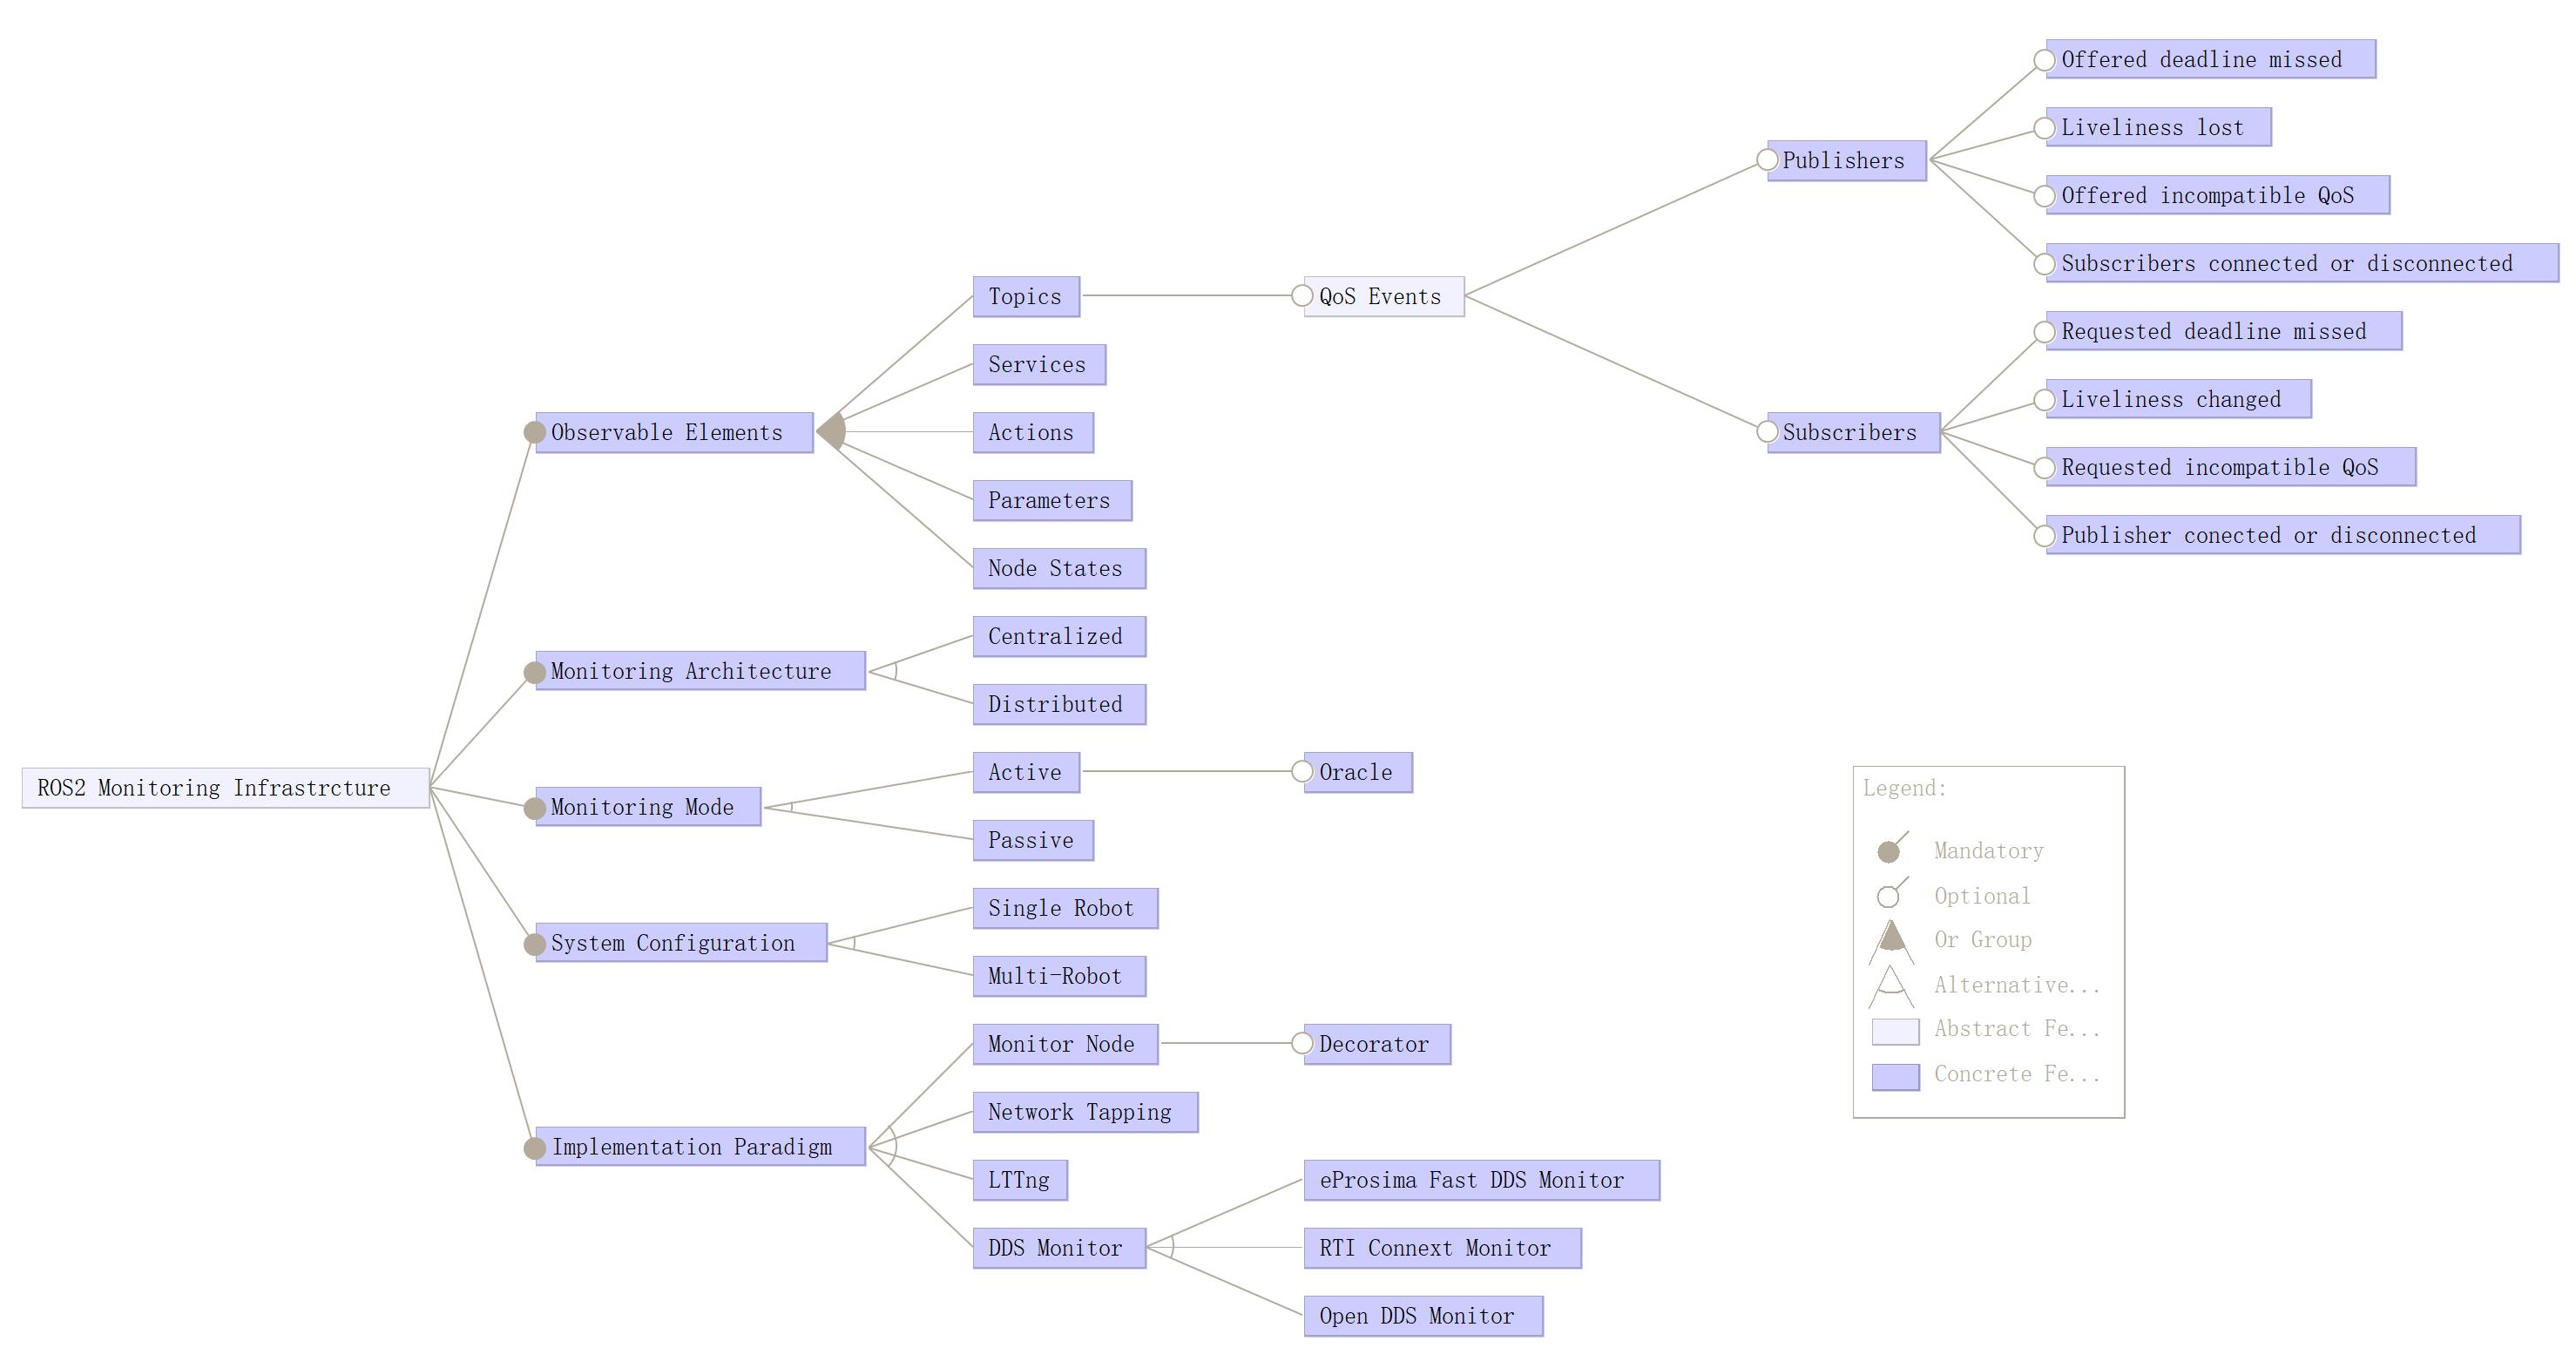
\includegraphics[width=1.0\linewidth]{Image/featureModel_Diagram.jpg}
    \caption{Diagram of Feature Model for ROS2 Monitoring Infrastructure}
    \label{fig:featuremodel}
\end{figure}

\vspace{0.3cm}

\textbf{Feature Relationships:}
\begin{itemize}[leftmargin=*]
    \item \textbf{Mandatory:} Must be included when parent is selected
    \item \textbf{Optional:} May not have to be selected
    \item \textbf{OR Group:} At least one must be selected
    \item \textbf{XOR Group:} Exactly one must be selected
\end{itemize}

\textbf{Cross-Tree Constraints:}
\begin{itemize}[leftmargin=*]
    \item \textbf{Multi-Robot $\rightarrow$ Distributed:} Multi-robot configurations require distributed monitoring architecture
    \item \textbf{Actions $\rightarrow$ (Topics $\land$ Services):} Action monitoring requires both topic and service monitoring since actions internally use both mechanisms
    \item \textbf{Decorator $\rightarrow$ Python Node:} The decorator implementation paradigm is only applicable to Python-based ROS2 nodes.
    \item \textbf{Network Tapping $\rightarrow$ $\lnot$Node States:} Network tapping operates at the DDS layer and cannot observe internal node states, which are not exposed over the network
    \item \textbf{(Network Tapping $\lor$ LTTng) $\rightarrow$ Passive:} Both network tapping and LTTng are inherently passive observation mechanisms that cannot actively inject monitoring probes into the system
\end{itemize}

\subsection{Use Case}
To validate the proposed monitoring infrastructure and address the research questions, this research utilizes the \textbf{Navigation 2 (Nav2)} stack as the primary System Under Verification (SUV). Nav2 is a industry-standard navigation framework for ROS 2, designed to enable mobile robots to move autonomously and safely. It is selected because it represents a ROS2 system that is widely adopted, open-source, and architecturally rich.

\begin{itemize}
    \item \textbf{Extensive use of Actions:} Unlike simple demonstrations that rely solely on Topics, Nav2 uses ROS 2 Actions (e.g., \texttt{NavigateToPose}, \texttt{FollowPath}) for its core behaviors. This supports the investigation of Action monitoring capabilities, addressing a key gap identified in existing approaches.
    \item \textbf{Strict Lifecycle Management:} Nav2 implements \textit{Managed Nodes} (Lifecycle Nodes) for its subsystems (Planner, Controller, Behavior Server). This provides a standardized environment to verify the infrastructure's ability to track Node States and transition events (e.g., \textit{Active}, \textit{Inactive}, \textit{Unconfigured}).
    \item \textbf{Scalability and Multi-Robot Support:} Nav2 natively supports multi-robot fleets through namespacing. This allows for the creation of complex distributed scenarios—such as swarms or warehouse fleets—to evaluate the performance trade-offs of the generated monitoring architecture.
\end{itemize}

\subsubsection{Validation Scenarios}
The monitoring infrastructure will be tested using three progressively complex scenarios within a Gazebo simulation environment:

\textbf{Scenario 1: Action Monitoring.}
As shown in Figure~\ref{fig:nav-task} and~\ref{fig:nav-obstacle}, the robot will execute navigation tasks using the capabilities provided by Nav2. During navigation, obstacles will be dynamically added using the Gazebo simulator. By comparing the information received by the Action Server with the information captured by the monitor, validating Action monitor can be generated effectively. Additionally, switching the target destination during execution will verify that monitor Action preemption can be captured.

\begin{figure}[H]
    \centering
    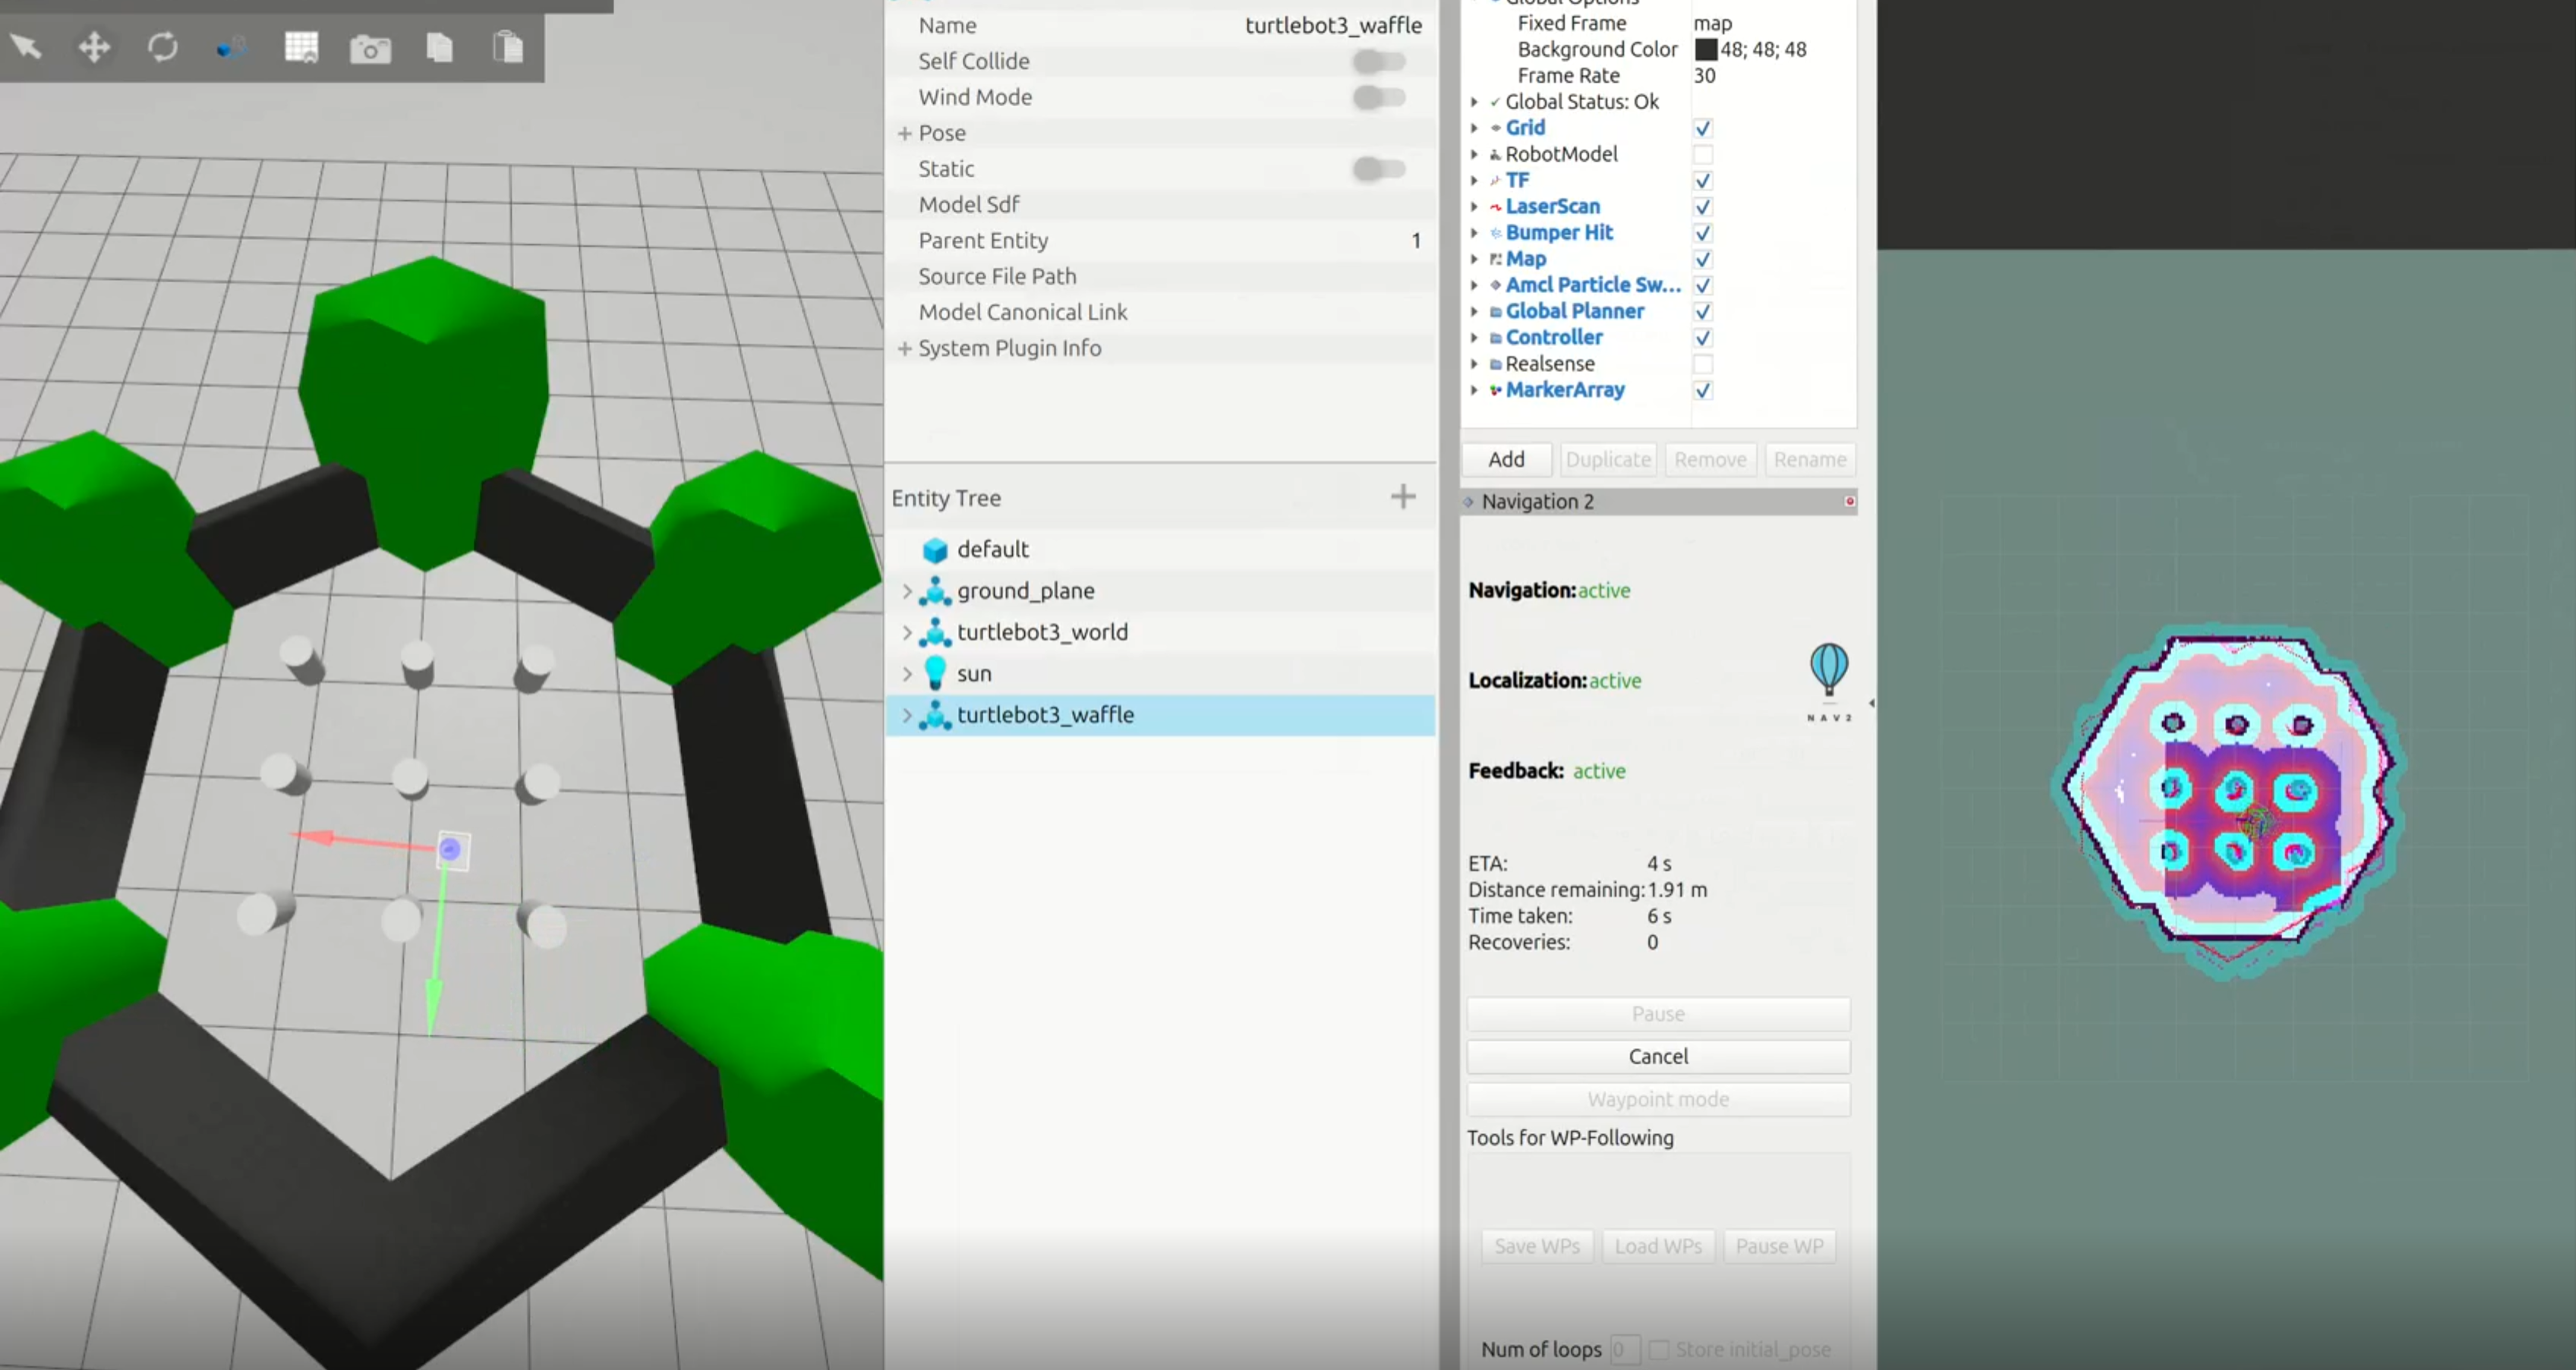
\includegraphics[width=0.85\linewidth]{Image/Figure3.png}
    \caption{Robot is performing a navigation task}
    \label{fig:nav-task}
\end{figure}

\begin{figure}[H]
    \centering
    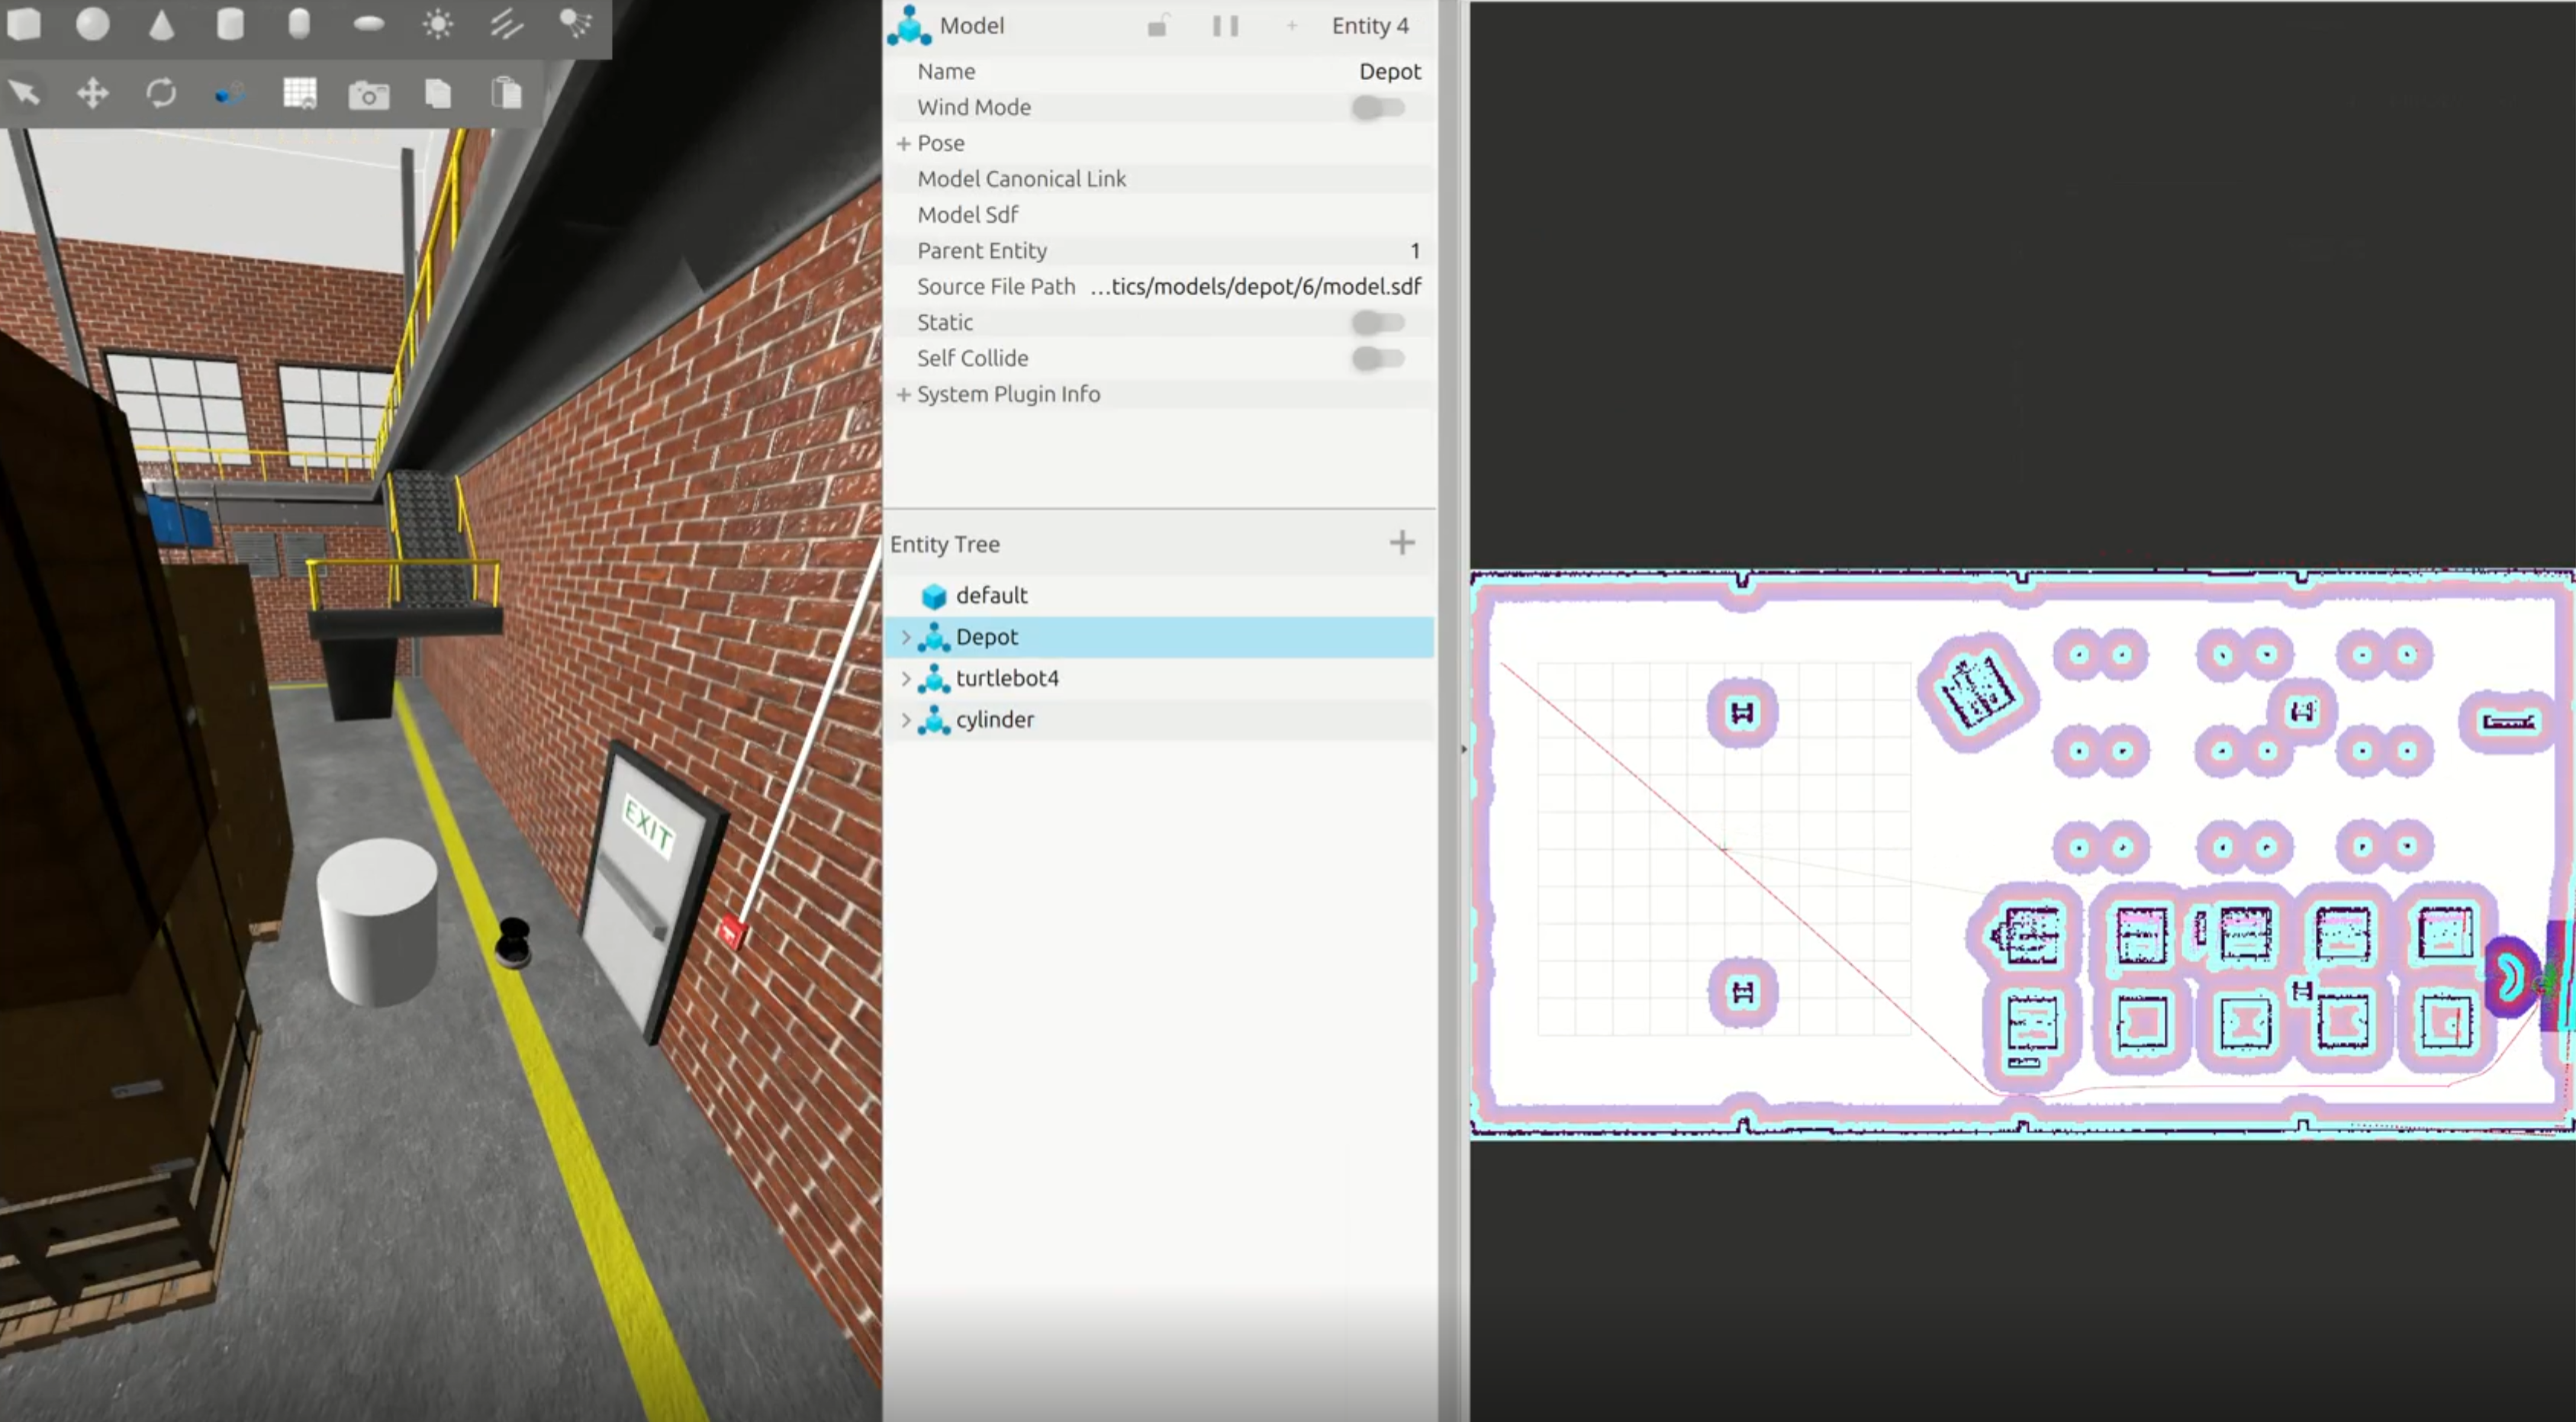
\includegraphics[width=0.85\linewidth]{Image/Figure4.png}
    \caption{An obstacle is placed along the robot's navigation path.}
    \label{fig:nav-obstacle}
\end{figure}

\textbf{Scenario 2: Lifecycle and Health Monitoring.}
A single robot will be deployed to verify the fundamental observation capabilities. The generated monitor will track the lifecycle transitions of the \texttt{controller\_server} and \texttt{planner\_server}. Additionally, it will monitor the \texttt{/bond} topic to detect heartbeat failures, verifying the system's ability to identify different status of nodes in ROS2 system.

\textbf{Scenario 3: Multi-Robot Collaboration.}
A collaborative scenario, like Figure~\ref{fig:multi-robot}, a ``Leader-Follower'' operation or a multi-robot warehouse task, will be implemented using two or more robots. The computational overhead differences will be compared by deploying different monitoring architectures (distributed vs. centralized).

\begin{figure}[H]
    \centering
    \includegraphics[width=0.85\linewidth]{Image/Figure5.png}
    \caption{Two robots are performing a collaborative task.}
    \label{fig:multi-robot}
\end{figure}

\newpage

% ============================================================================
\section{Project Plan and Risks}
\label{ch:planrisk}
% ============================================================================

\subsection{Project Plan}

The goal is this project starts in March 2026 and ends with graduation in August 2026.


\begin{figure}[H]
    \centering
    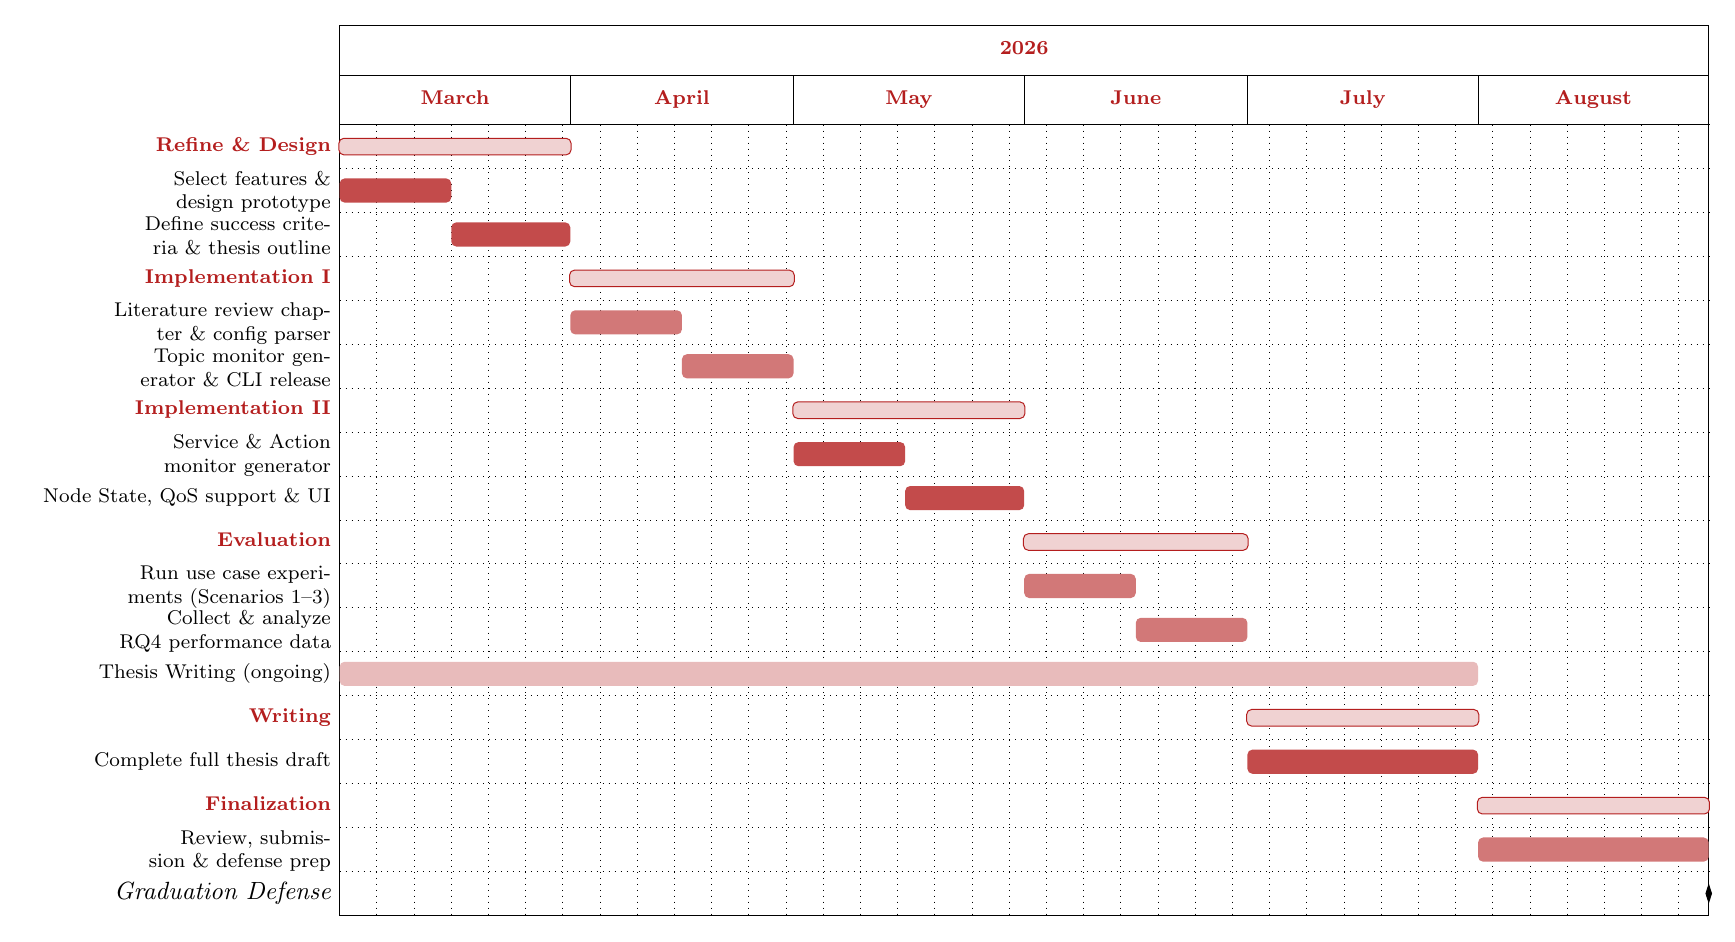
\includegraphics[width=1.0\linewidth]{Image/plan_gantt.png}
    \caption{Project Plan}
    \label{fig:placeholder}
\end{figure}



\subsection{Threats to Validity}
\begin{itemize}[leftmargin=*]
    \item \textbf{Lab Test:} Internal validity may be limited, due to the experimental evaluation will be conducted in a simulated environment, which may not fully reflect real-world operating conditions.
    \item \textbf{Sample size:} Test scenarios are limited, which may affect the statistical reliability of the results.
    \item \textbf{Generalization:} External validity may be limited because the system will be evaluated only using the Nav2 framework, and the findings of performance overhead may not generalize to other ROS2 systems.
    \item \textbf{Middleware Dependency:} ROS2 supports multiple middleware providers (e.g., Fast DDS, Cyclone DDS), the performance overhead of the generated monitors may vary across different middleware configurations.
    \item \textbf{Performance Noise:} It might be hard to distinguish between the performance overhead used by Nav2 and by the monitor.
    \item \textbf{Version Sensitivity:} The implementation and evaluation depend on specific versions of ROS2, Nav2, and Gazebo. Behavioral differences across versions may affect the reproducibility of the results.
    \item \textbf{Code Generator Coverage:} The code generator is tested against a limited set of Feature Tree configurations. As the full configuration space is combinatorially large, untested combinations may not behave correctly.
    \item \textbf{Specification Bias:} The Feature Tree is constructed based on a literature review and the author's own analysis. If relevant observable elements or configuration options are overlooked, the results will inherit these blind spots.

\end{itemize}

\subsection{Risks}
\begin{itemize}[leftmargin=*]
    \item \textbf{Time Constraint:} There may not be sufficient time to complete a sufficiently versatile monitoring infrastructure generator. To mitigate this, the project plan prioritizes core functionality (Topic and Action monitoring) before extending to optional features.
    \item \textbf{Tooling Dependency:} The project depends on the stability of ROS2, Nav2, and Gazebo. Breaking changes in upstream packages could delay progress. Pinning specific versions of all dependencies will reduce this risk.
    \item \textbf{Simulation Fidelity:} Gazebo simulation may introduce artifacts (e.g., timing jitter, unrealistic sensor noise) that affect the validity of performance measurements. Where possible, results will be cross-validated with analytical expectations.
\end{itemize}

% ============================================================================
\section{Conclusion}
% ============================================================================

This project addresses the need for configurable monitoring infrastructure at the foundation layer of ROS2 monitoring frameworks. By taking a bottom-up approach, the project establishes the essential capability to collect observations from ROS2 systems through automatically generated monitoring infrastructure. The configuration-based approach allows users to specify their monitoring requirements declaratively and obtain ready-to-deploy monitoring nodes without manual instrumentation.

This foundation layer provides the groundwork for future work on data abstraction and specification-based evaluation, enabling the development of a complete, layered monitoring framework for ROS2 applications.

\newpage

\bibliographystyle{IEEEtran}
\bibliography{General/References.bib}

\end{document}